\documentclass[a4paper,10pt]{article}
\usepackage{etex}
\usepackage[spanish,es-noquoting]{babel}
\usepackage[utf8]{inputenx}
\usepackage{booktabs}
\usepackage{multirow}
\usepackage{amssymb}
\usepackage{graphicx}
\usepackage{listings}
\usepackage{verbatim}
\usepackage{diagrams}
\usepackage{proof}
\usepackage{amsmath}
\usepackage[all,color]{xy}
\newcommand{\here}{\checkmark}

\newenvironment{code}{\footnotesize\verbatim}{\endverbatim\normalsize}
\DeclareUnicodeCharacter{03BB}{$\lambda$}
\DeclareUnicodeCharacter{2192}{$\rightarrow$}

\usepackage{tikz}
\usetikzlibrary{arrows}

\tikzset{
  treenode/.style = {align=center, inner sep=0pt, text centered,
    font=\sffamily},
  arn_n/.style = {treenode, circle, white, font=\sffamily\bfseries, draw=black,
    fill=black, text width=1.5em},% arbre rouge noir, noeud noir
  arn_r/.style = {treenode, circle, red, draw=red, 
    text width=1.5em, very thick},% arbre rouge noir, noeud rouge
  arn_x/.style = {treenode, rectangle, draw=black,
    minimum width=0.5em, minimum height=0.5em}% arbre rouge noir, nil
}

\newcommand{\typejud}[3] {
  \ensuremath{#1 \vdash #2 : #3}
}

\newcommand{\df}[1]{\textcolor{gray}{\mathsf{#1}}}
\newcommand{\dfH}[1]{\textcolor{blue}{\mathsf{#1}}}

\title{Language Implementation: Attribute Grammars}
\author{Alejandro Gadea \and Emmanuel Gunther}

\begin{document}
\maketitle
\lstset{ language=Haskell
       , literate={λ}{{$\lambda$}}1{→}{{$\rightarrow$}}1
	   }

\section{Syntax and Semantics of Languages}

\subsection{The RepMin problem}

The ``Rep Min'' is a well known example of the expressiveness of Lazy Evaluation and
inspires the way to define the semantics that exploit the Attribute Grammars.

Think about the data type of binary trees, with numbers in the leaves. The problem
consists in replacing each value at each leaf by the least value if the whole tree:\\

\begin{minipage}{.37\textwidth}
\begin{tikzpicture}[level/.style={sibling distance = 3cm/#1,
  level distance = 0.7cm}] 
\node [arn_n] {}
    child{ node [arn_r] {4} }
    child{ node [arn_n] {}
            child{ node [arn_n] {} 
							child{ node [arn_r] {3}}
							child{ node [arn_r] {10}}
            }
            child{ node [arn_r] {4} }
		}
;
\end{tikzpicture}
\end{minipage}%
\begin{minipage}{.18\textwidth}
\begin{tikzpicture}
\coordinate (a) at (0,0);
\coordinate (b) at (2,0);
\draw[-angle 90, red!40!white, line width=9pt](a) to node[black]{rep\_min} (b) ;
\end{tikzpicture}
\end{minipage}
\begin{minipage}{.2\textwidth}
\begin{tikzpicture}[level/.style={sibling distance = 3cm/#1,
  level distance = 0.7cm}] 
\node [arn_n] {}
    child{ node [arn_r] {3} }
    child{ node [arn_n] {}
            child{ node [arn_n] {} 
							child{ node [arn_r] {3}}
							child{ node [arn_r] {3}}
            }
            child{ node [arn_r] {3} }
		}
;
\end{tikzpicture}
\end{minipage}

\

\

We can define a data type in Haskell for representing a binary tree in the following way:

\begin{lstlisting}
 data Tree =   Leaf Int 
	     | Bin (Tree,Tree)
\end{lstlisting}

A tree can be built from an integer (a leaf) or from others two subtrees, i.e we
can think of an element of $Tree$ as an element of the disjoint union of 
$Int \sqcup (Tree\,\times\,Tree)$. This disjoint union can be defined for any
type $a$:

\begin{lstlisting}
 type FTree a = Either Int (a,a)
\end{lstlisting}

\noindent and then we can get any element of $\mathbf{Tree}$ from some element
of $\mathbf{FTree\,Tree}$.

AS we will see the type of that function is interesting in itself, so we explicitly
define it:

\begin{lstlisting}
 type FTreeAlgebra a = FTree a -> a
\end{lstlisting}

Now, if we want to define a semantics for the binary trees in the semantic set $B$ we can
define a $\mathbf{FTreeAlgebra}\;B$. This is, we should give a rule in the case of having
an integer and another in the case of having a pair in $B \times B$, which one should think
as the semantic value of the subtrees.

For example, the syntactic representation of binary trees with the type $Tree$ could be
the trivial semantics as follows:

\begin{lstlisting}
  init_algebra :: FTreeAlgebra Tree
  init_algebra = either Leaf Bin
\end{lstlisting}

Thinking in categories, we can see $FTree$ as a functor which transform an object $A$ in
an object $Int \uplus (A \times A)$ and then a FTree-algebra will be an arrow 
$\alpha\,:\,FTree\;A \rightarrow A$. If $\alpha$ is the initial FTree-algebra, then for
any other FTree-algebra $\beta\,:\,FTree\;B \rightarrow B$ there must exist an unique arrow
between $\alpha$ and $\beta$, i.e, a single $f$ such that the following diagram commutes:

\begin{center}
\begin{diagram}
   FTree \ A & & \rTo^{\alpha} & & A \\
   \dTo^{FTree \ f} & & & & \dTo_{f} & \\
   FTree \ B & & \rTo^{\beta} & & B &
\end{diagram}
\end{center}

\

\

Thus, if we want to define a semantics for the binary trees we must find the single arrow
between the $init\_algebra$ (the initial FTree-algebra) and other FTree-algebra. This arrow
is called \textbf{catamorfism}:

\begin{lstlisting}
  cataTree :: FTreeAlgebra b -> Tree -> b
  cataTree beta (Leaf i)    = beta (Left i)
  cataTree beta (Bin (t1,t2)) = beta (Right (cataTree beta t1,
					     cataTree beta t2))
\end{lstlisting}

Let us return to the problem that we want to solve, given a tree we want to transform it
in the tree in which the value of the leaves is the least value.

In a first attempt, we get the least value of the tree and then replace it in
all the leaves. This implies walking the initial tree two times.

Now, to get the least value we define a FTree-algebra and define a function that
given an integer $n$ constructs the FTree-algebra which replace the value of the leafs
for $n$, the least value got in the first phase:

\begin{lstlisting}
  min_alg :: FTreeAlgebra Int
  min_alg = either id (uncurry min)

  rep_min_alg :: Int -> FTreeAlgebra Tree
  rep_min_alg n = either (const $ Leaf n) Bin
\end{lstlisting}

Finally, we solve the problem calling twice the function $cataTree$:

\begin{lstlisting}
  replace_min :: Tree -> Tree
  replace_min t = let n = cataTree min_alg t in
		      cataTree (rep_min_alg n) t
\end{lstlisting}

Notice that in the function $rep\_min\_alg$ we have an FTree-algebra from a integer.
Instead of doing this, we can define an FTree-algebra which allow us to compute a
function that given an integer builds up a tree with all the values of the leafs
replaced by the integer:

\begin{lstlisting}
  rep_min_alg' :: FTreeAlgebra (Int -> Tree)
  rep_min_alg' = either (const Leaf) 
                        (\(lfun,rfun) -> \m -> 
			    Bin (lfun m,rfun m))
\end{lstlisting}

\noindent then, the solution to our problem can be stated as:

\begin{lstlisting}
  replace_min' :: Tree -> Tree
  replace_min' t = (cataTree rep_min_alg' t) (cataTree min_alg t) 
\end{lstlisting}

In the last definition we can see that the calls to the function $cataTree$ are independent, thus
we could compute a single FTree-algebra that get both results at the same time. With $min\_alg$
making the least value and with $rep\_min\_alg'$ the function for builds up the tree, therefore if
we could make the product of those FTree-algebra we would get both results:

\begin{lstlisting}
  infix 9 `x`

  x :: FTreeAlgebra a -> FTreeAlgebra b -> FTreeAlgebra (a,b)
  fa `x` fb = either  (\i -> (fa $ Left i,fb $ Left i))
		      (\((a,b),(a',b')) -> 
			(fa $ Right (a,a'),fb $ Right (b,b')))
			  

  rep_min_alg'' :: FTreeAlgebra (Int,Int -> Tree)
  rep_min_alg'' = min_alg `x` rep_min_alg'
  
\end{lstlisting}

So now we can get the result to the problem making only one call to $cataTree$:

\begin{lstlisting}
 replace_min'' :: Tree -> Tree
 replace_min'' t = r m
    where (m, r) = cataTree rep_min_alg'' t
\end{lstlisting}

One final improvement can be considered, for this we introduce the following
function that given two isomorphic types $a$ and $b$, and a $FTreeAlgebra\;a$ 
constructs a $FTreeAlgebra\;b$:

\begin{lstlisting}
getIsoAlg :: (a -> b) -> (b -> a) -> FTreeAlgebra a -> FTreeAlgebra b
getIsoAlg fab fba fa = either (fab . fa . Left)
                                 (fab . fa . Right . (fba *** fba))
\end{lstlisting}

In our problem we have a FTree-algebra of type
  
\begin{lstlisting}
   (Int,Int -> Tree)
\end{lstlisting}

and we can consider, for our problem, that it is equivalent to the type
(explain this, Ah! traducía todo... :) )

\begin{lstlisting}
Int -> (Int,Tree)
\end{lstlisting} 

Then, we need two functions to exchange those types such that they are one inverse to the other:
  
\begin{lstlisting}
f1 :: (Int,Int -> Tree) -> (Int -> (Int,Tree))
  
f2 :: (Int -> (Int,Tree)) -> (Int,Int -> Tree)
\end{lstlisting}

The first we can construct easily, but that is not the case for the second one. We find that to
get the first element of the pair we don't know which value give to the function:

\begin{lstlisting}
f1 :: (Int,Int -> Tree) -> (Int -> (Int,Tree))
f1 (i,f) = const i &&& f

f2 :: (Int -> (Int,Tree)) -> (Int,Int -> Tree)
f2 f = (??? , snd . f)
\end{lstlisting}

we must follow... (seguía traduciendo de mas ja)

% de los árboles binarias con el tipo $Tree$ constituyen el álgebra inicial, que consiste en
% aplicar la función $Leaf$ si el elemento es un entero, y la función $Bin$ si 

\subsection{Repmin with Attribute Grammars}

In the previous section we saw how to solve the problem of Repmin in a more efficient way, performing
a single walk thanks to the Lazy Evaluation of Haskell. For this we obtain a tuple in
which the first element was the least value of the tree and the second one was a function that
given an integer builds up a tree with all the values of the leafs of the tree replaced for
the integer.

Notice that we could take the same steps for any other recursive data type, where the grammar
not necessarily has two productions. We could define a functor $F$ and the appropriate catamorphism,
and then for calculating any semantics we only need to give one rule for each production of the
grammar.

With \textbf{Attribute Grammars}, we have a simple notation for specifying a semantics, defining the
syntax of a data type and then to give the rules for each production of the grammar. A preprocessor
transform the AG notation to Haskell code that is equivalent to that obtained in the previous
section.

Let us illustrate this point showing how the Repmin problem can be solved with AG:

\begin{lstlisting}
data Tree
    | Leaf      Int
    | Bin lt :: Tree
	      rt :: Tree

deriving Tree : Show
	  
attr Tree
    inh minval :: Int
    syn m      :: Int
    syn res    :: Tree
      
sem Tree
    | Leaf lhs.m   = @int
              .res = Leaf @lhs.minval
	| Bin  lhs.m   = @lt.m `min` @rt.m
              .res = Bin @lt.res @rt.res

data Root
	| Root Tree
      
      
attr Root
	syn res :: Tree
      
sem Root
	| Root tree.minval = @tree.m
\end{lstlisting}

The definition of the grammar is similar to the one given in Haskell, the only difference is that we 
just put names in each parameter of each production. To calculate the semantics we define two kinds of 
attributes, the synthesised ($syn$), which are those that for computing the value in a node we need to 
know the value of the childrens, and the inherited ($inh$), which are passed top to down in the tree.

In our example we need the least value of the tree to compute the result of Repmin, then we define
an inherited attribute $minval$ and two synthesized attributes, $m$ to calculate the least value
of the tree and $res$ to compute the final tree with the replaced of $minval$ that is initialized
in $m$.
  
In the previous piece of code we used many abbreviations that allows us to write shorter code.
For example, if a rule of a grammar production has a single argument, we can be omit the definition of
the name and the preprocessor generates one consistent one with the name of the data type which has the
first letter in lowercase. If an inherited attribute doesn't change the value passed to the children
nodes, then it's not necessary to define that trivial rule.

The generated code using \textbf{Attribute Grammars} computes the attributes values by doing the
procedure that we have show in the previous section. The type of the resulting algebra will be a function
where the parameters are the inherited attributes and the result will be a tuple where each element
is a synthesized attribute.
  
%   En general podemos tener muchos problemas donde necesitemos calcular algunos valores en una estructura de datos
%   que luego tengan que ser utilizados para calcular otros valores, con estructuras recursivas más complicadas
%   que los árboles binarios. Realizar todo el proceso que mostramos puede ser tedioso y propicio para cometer
%   errores

\section{The Lambda Calulus}

In the previous section we saw how we can define a function in a general way, we called
catamorphism, and how this is internalized in the AG framework with a special syntax
with the idea that we just need to implement the relating things of the problem.

In the following, we will implement a type inference algorithm for the simply typed lambda
calculus, as well as the parser and the pretty printer.

\subsection{Syntax: Parser y Pretty Printing}

\subsubsection{Syntax}

Let $Var$ be a countable set. In general, we will use $a$, $b$, $c$, $s$, $x$, $y$, $z$. To
denote elements of $Var$.

\begin{lstlisting}
Term ::= Var
       | λ Var . Term
       | Term Term
\end{lstlisting}

\subsubsection{Parser}

The implementation of a parser for the syntax of the lambda calculus is rather simple,
even adding the restriction that we only allow to parse closed terms, i.e. terms in which
don't occur free variables. However, suppose we should to parse the following string,\\

$\lambda a . s$\\

clearly ``s'' is free, but it would not be wrong to assume that the intended string was\\

$\lambda a . a$\\

i.e. a mistake was made by writing the string. Thus, a parser a little bit
more interesting would be one that detects that kind of errors, corrects them
and gives information about such decision.

For the implementation of the parser we use the library ``uu-parsinglib''
which provides exactly an error correction mechanism. For example, being ``pa'' the
parser of the letter ``a'', trying to parse ``b'' will produce an ``a'' the correction
being the replacement of ``b'' for ``a'':

\begin{code}
 >>> run pa  "b"
     Result: "a"
     Correcting steps: 
       Deleted   'b' at position LineColPos 0 0 0 expecting 'a'
       Inserted  'a' at position LineColPos 0 1 1 expecting 'a'
\end{code}

We would like to highlight that the error correction that we pretend for our parser
of terms comes almost for free. In a preliminary summary, for parsing the body of an 
abstraction we just need to have a list with the introduced variables till that
moment and generate parsers for each variable in the list.\\

Before introducing the parsers concerning each construction of the grammar, 
we define some general parsers that will be useful.

\begin{lstlisting}
parseTermSym :: Parser String -> [String] -> Parser String
\end{lstlisting}
We generate a parser from a default parser and a list of strings.

\begin{lstlisting}
parseXSym :: Parser String
\end{lstlisting} with X $\in$ {Lam,Dot,App}\\
Parsers for the symbols $\lambda$, $.$ and $@$. Further we can
parser ``\textbackslash \textbackslash'' instead of $\lambda$ and $->$ or $\rightarrow$
instead of ``$.$'' .

\begin{lstlisting}
parseVar :: Parser Var
\end{lstlisting} Parser for variables.\\

Now, given the list of variable to parse, say $vars$, identifier
we generate parsers for each variable in the list and fail as default parser:

\begin{lstlisting}
parseId :: [Var] -> Parser Term
parseId vars = Id <$> parseTermSym pFail vars
\end{lstlisting}

Something interesting to highlight is that we include the correcting action in
the generated parser for variables.\\

For the case of the abstraction, leaving aside the parsing of the respective symbols,
we are going to parse a variable and we could say that we need two things;
(1) the constructor of the abstraction, (2) the list of possibles variables to parse.
This brings a problem, since when we parse a variable this is encapsulated inside
of the computation ``Parser Var'', by (2) we can think that the type of the parser
that parse the body of the abstraction should be $Var -> Parser Term$, because it takes the
variable, adds it to the list of bound variables and then parse the term.

If we pay attention we need a function which takes a parser for the bound occurrence,
the function expecting that variable and parses the body adding the variable to the
list of bound variables, i.e. a function with type:

\begin{lstlisting}
Parser Var -> (Var -> Parser Term) -> Parser Term
\end{lstlisting}

but this is just the type of the bind operator ($>>=$), $m \ a \rightarrow (a \rightarrow m \ b) \rightarrow m \ b$. This forces us to use monads, for which we need to use the addLength function.
We are not sure if there exist a way to solve this without monads, with the purpose of avoiding the
use of addLength and of course... monads. Then, the final definition is,

\begin{lstlisting}
parseAbs :: [Var] -> Parser Term
parseAbs vars = 
       addLength 1 $
       join $ uncurry (<$>) 
           <$> 
       (Abs &&& parseTerm . (:vars))
       	   <$ 
       parseLamSym <*> parseVar <* parseDotSym
\end{lstlisting}

For concluding, for the case of the application we try to parse bound variables, abstractions
or applications, for which we use the symbol ``$@$'', this parser is defined as follows,

\begin{lstlisting}
parseTerm' :: [Var] -> Parser Term
parseTerm' vars =  parseId vars
               <|> parseAbs vars
               <|> pParens (parseTerm vars)

parseApp :: [Var] -> Parser Term
parseApp vars = (App <$ parseAppSym) `pChainl` (parseTerm' vars)
\end{lstlisting}

then, parsing a term is simply the parsing of an application,

\begin{lstlisting}
parseTerm :: [Var] -> Parser Term
parseTerm vars = parseApp vars
\end{lstlisting}

In conclusion, we have a parser for the grammar of the lambda calculus which also corrects some
mistakes, as we mentioned at the beginning. Something important to comment is that the
correction of errors may have some unwanted behaviour due to the ``simplistic''
implementation using the internal mechanisms of corrections offered by the library. An example
of this may be,

\begin{verbatim}
>>> parserTerm "\\a -> b@a"
(λ a → a
, [-- Deleted   'b' at position LineColPos 0 6 6 expecting Whitespace
  ,-- Deleted   '@' at position LineColPos 0 7 7 expecting "a"
  ]
)
\end{verbatim}

where most probably the wanted correction it would be the replacement of ``b'' for
``a'', and the production of the term $\lambda$ $a$ $\rightarrow$ $a@a$.

\subsubsection{Pretty Printing}

The implementation of the pretty printing is of interest to us as a first little step to
the definition of the semantic function for the data type $Term$ using AG. In
summary, the semantics we are thinking transforms a $Term$, i.e. a term
of the lambda calculus, in his representation in $String$.\\

Despite of having few constructors, a term of the lambda calculus can be complex
to read and an ``organization'' of the subterms when it comes to writing can be
very helpful for the interpretation. For example, the term 
$(\lambda x \rightarrow x@x)@(\lambda x \rightarrow x@x)$
does not bring much trouble, but however if we have,
$(\lambda x \rightarrow
	\lambda y \rightarrow
		\lambda f \rightarrow f @ (x @ (\lambda w \rightarrow f @ w)) @ (y @ f @ x))$
$@$
$(\lambda x \rightarrow 
	\lambda y \rightarrow \lambda f \rightarrow 
	\lambda g \rightarrow \lambda h \rightarrow h @ (f @ x) @ (g @ y))$
$@$ $\lambda x \rightarrow \lambda f \rightarrow 
		\lambda g \rightarrow f @ g @ (x @ g)$
it is certainly more difficult to read. Thus, a good presentation of the term can be always
helpful. The use of the ``uulib'' library, in particular ``UU.PPrint'', gives us
a way of implement a pretty printer in a simple way.

As we saw for the case of Repmin, we must define attributes and give rules for
each constructor, this time for $Term$, which express how to transform each of its productions
in its representation as strings.

We want a synthesised attribute, that called ``pprint'', that is the result
of transforming a $Term$ in a $String$ and an inherited attribute that we need to
know when to enclose a term between brackets or not.

\begin{lstlisting}
attr Term 
    syn pprint :: {Doc}
    inh paren  :: {ParenInfo}
\end{lstlisting}

\noindent On the other hand the semantic is defined as,

\begin{lstlisting}    
sem Term
\end{lstlisting}
Pretty-printing a variable consists sumply in printing the name
\begin{lstlisting}    
    | Id  lhs.pprint  = text @ident
\end{lstlisting}

In the case of the application, we began explaining that to print an application will
be as simple  as printing its left side (lt) and its right side (rt) but taking into account 
some considerations; as for the brackets, because the application is left associative if we
have, for example the application of $x@y$ to $z@w$ we will need to place parenthesis only in the right side ($rt.paren = Paren$) for printing the correct application $x@y@(z@w)$. But also, there is
a particular case where the left side needs to be enclosed in parentheses, for example
applying $\lambda x \rightarrow x$ to $z@w$. That is the reason for putting parenthesis
around the left side only when it is an abstraction ($lt.paren = ParenAbs$).
Notice that without the parenthesis in the example, applications would be $x@y@z@w$ and
$\lambda x \rightarrow x@z@w$ which are not the correct representations of the original
terms.

Now, leaving aside parentheses, for printing an application the idea would be to try that
both sides, the operator and the operand, stay at the same level and in the case that this is not
possible obtain the following,

\begin{center}
$lt$\\
$@$\\
$rt$
\end{center}

i.e, to divide the subterms in two levels intercalating the application operator. With the
possibility of putting the right side at the same level of the operator.

\begin{lstlisting}    
    | App lhs.pprint  = (putParen @lhs.paren) 
                (group $ @lt.pprint <> line <> 
                  (group $ text "@" <> line <> @rt.pprint)
                )
          rt.paren    = Paren
          lt.paren    = ParenAbs
\end{lstlisting}    

To finish, we need to define the semantics for the case of the abstraction constructor.
For this case the idea is to write all the abstraction i the same level; but, when it
does not fit, we will print the body ($term$) in other level with some
indentation (3 characters) to ease the reading of the body, when the abstraction is applied
to other term. On the other hand, the body of the abstraction never
needs to be between parentheses ($term.paren = NoParen$).

\begin{lstlisting}
    | Abs lhs.pprint  = (putAbsParen @lhs.paren)
                (text "λ " <> text @var <> text " →" <> 
                    group (nest 3 $ line <> @term.pprint)
                )
          term.paren  = NoParen
\end{lstlisting}

Printing the example of the beginning with our pretty-printer, we can note that it is much easier 
to read. In particular, it contains many of the print cases that the semantics we give implements.

\begin{verbatim}
>>> App (App t2 t3) t1
(λ x →
   λ y →
      λ f → f @ (x @ (λ w → f @ w)) @ (y @ f @ x))
@
(λ x →
   λ y → λ f → λ g → λ h → h @ (f @ x) @ (g @ y))
@ (λ x → λ f → λ g → f @ g @ (x @ g))
\end{verbatim}

\subsection{Inferidor de tipos}
 El objetivo principal de este trabajo es realizar un inferidor de tipos para el cálculo lambda con tipos simples. Recordemos
 las reglas de tipado:
 
 \begin{align*}
 \infer[^{\mathtt{T-VAR}}]
       {\typejud{\pi,(v:\theta)}{v}{\theta}}
       {}
 \end{align*}
  \begin{align*}
  \infer[^{\mathtt{T-APP}}]
       {\typejud{\pi}{t_1\;t_2}{\theta_2}}
       {\typejud{\pi}{t_1}{\theta_1\rightarrow\theta_2} &
        \typejud{\pi}{t_2}{\theta_1}
       }
  \end{align*}
  \begin{align*}
  \infer[^{\mathtt{T-ABS}}]
       {\typejud{\pi}{\lambda\,v.t}{\theta_1 \rightarrow \theta_2}}
       {\typejud{\pi,(v:\theta_1)}{t}{\theta_2}
       }
  \end{align*}
 
 En un contexto $\pi$ un término $t$ tendrá tipo $\theta$ si existe una derivación de
 $\typejud{\pi}{t}{\theta}$ utilizando las reglas anteriores.
 
 Para inferir el tipo de un término lo que podemos hacer es asumir que tiene un tipo $\theta$, e ir anotando
 substituciones a ese tipo hasta obtener un juicio de tipado válido. Supongamos que tenemos el siguiente término:
 
 \begin{align*}
    \lambda\,x.x
 \end{align*}

  Asumimos que tiene tipo $\theta$, pero como es una abstracción la única regla con la que podemos construir un juicio
  válido es $\mathtt{T-ABS}$ donde concluye que el tipo tiene que ser de la forma $\theta_1 \rightarrow \theta_2$, 
  por lo tanto agregaríamos la substitución $\theta\,:=\,\theta_1 \rightarrow \theta_2$ y luego
  intentamos construir el juicio de tipado $\typejud{\pi,(x:\theta_1)}{x}{\theta_2}$, como el término ahora
  es una variable la única regla posible es $\mathtt{T-VAR}$ para lo cual necesitamos agregar
  la substitución $\theta_1\,:=\,\theta_2$, y finalmente el tipo inferido es
  
  \begin{align*}
   \typejud{\empty}{\lambda\,x.x}{\theta_2 \rightarrow \theta_2}
  \end{align*}

  Con esta idea realizaremos la inferencia de tipos utilizando Attribute Grammars. Definimos la gramática:
  
  \begin{lstlisting}
   data Term
	| Id  ident :: {Var}
	| App lt,rt :: Term
	| Abs var   :: {Var}
	      term  :: Term
  \end{lstlisting}

  Donde $Var$ está definido como $String$.
  
  Y los siguientes atributos:
  
  \begin{lstlisting}
   attr Term 
      inh ctx       :: {Ctx}
      inh termType  :: {Type}
      inh usedTVars :: {S.Set TVar}
      syn tsubst    :: {TSubst}
  \end{lstlisting}

  El resultado de la inferencia de tipos será una substitución a aplicar sobre el tipo inicial, y lo implementamos con 
  un atributo sintetizado $\mathbf{tsubst}$. Como vimos en el ejemplo anterior, dado un término asumimos que tiene un 
  tipo determinado, ese tipo asumido está implementado con un atributo sintetizado $\mathbf{termType}$. Tendremos
  también un contexto de asignación de tipos a las variables con el atributo $\mathbf{ctx}$, y como necesitaremos generar
  variables de tipos frescas cada vez que asumimos un nuevo tipo, llevamos cuenta de las variables de tipo ya usadas
  con el atributo $\mathbf{usedTVars}$.
  
  Para ver el funcionamiento del algoritmo implementado con Attribute Grammars consideremos el siguiente término 
  sobre el cual inferir el tipo:
  
 \begin{align*}
    \lambda\,f.\lambda\,x.f\;(f\;x)
 \end{align*}

 \noindent que con la gramática definida quedaría representado por
 \begin{lstlisting}
  Abs "f" (Abs "x" (App (Id "f") (App (Id "f") (Id "x"))))
 \end{lstlisting}
 
 \noindent o en forma de árbol:
 
  \begin{center}
  \begin{diagram}[h=2em]
	  & Abs \\
	  & \dTo_{f}\\
	  & Abs \\
	  & \dTo_{x}\\
	  & App\\
	  \ldTo(1,2) & & \rdTo(1,2)\\
	  f & & App\\
      & \ldTo(1,2) & & \rdTo(1,2)\\
	  & f & & x
  \end{diagram}
  \end{center}


  El primer nodo de este árbol es una abstracción. Tenemos que definir entonces el valor de los atributos heredados en
  el nodo hijo y calcular el atributo sintetizado en función del mismo.

\begin{center}
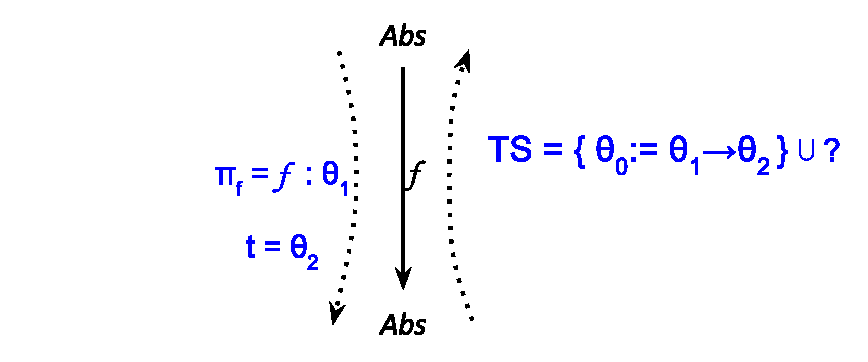
\includegraphics[height=4cm]{./primero.pdf}
\end{center}

   Como el tipo que habíamos asumido para este término es $\theta$ tendremos que substituirlo por $\theta_1 \rightarrow \theta_2$
   y entonces el contexto del subtérmino tendrá el par $f : \theta_1$, el tipo asumido será $\theta_2$ y agregamos a las variables
   usadas $\theta_1$ y $\theta_2$. La substitución contendrá $\theta : \theta_1 \rightarrow \theta_2$ más la substitución del 
   subtérmino. En los gráficos iremos completando la substitución a medida que calculamos los atributos de los subtérminos.
   
   
   
   En el siguiente paso, el nodo que analizamos es también una abstracción, por lo tanto repetimos el mismo procedimiento:
   
\begin{center}
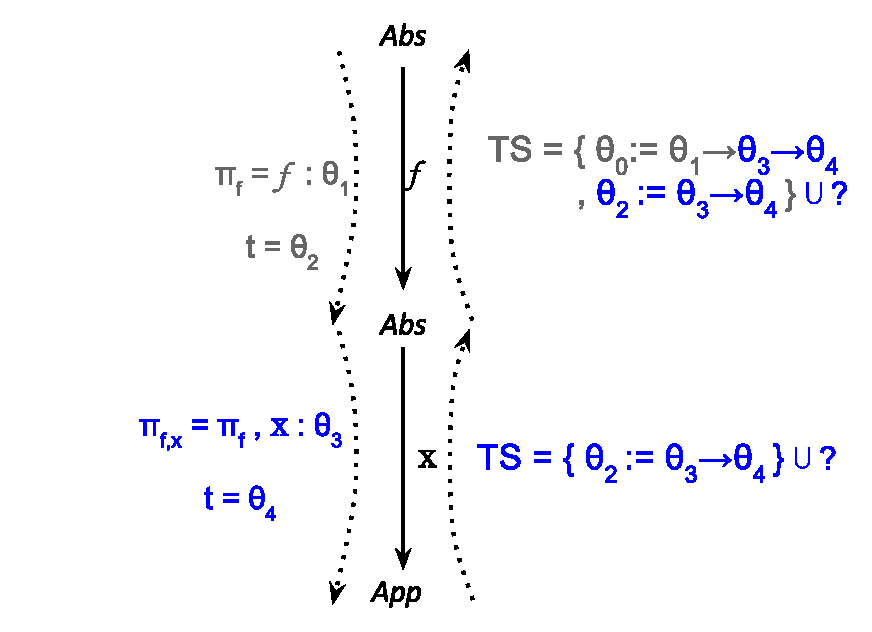
\includegraphics[height=8cm]{./segundo.pdf}
\end{center}

  \noindent $\theta_2$ será substituido por $\theta_3 \rightarrow \theta_4$, al contexto le agregamos $x:\theta_3$ y agregamos
  las nuevas variables a las usadas. El tipo que le asignamos al subtérmino es $\theta_4$. La substitución del nodo inicial
  la actualizamos en el gráfico agregando la obtenida en este subtérmino, y al hacerlo realizamos el reemplazo 
  $\theta_2 := \theta_3 \rightarrow \theta_4$, de esta manera aseguramos que las variables de tipo que ocurren al lado
  izquierdo no ocurren al lado derecho de la substitución. También al hacer la unión realizamos unificación de tipos en
  caso de ser necesaria.
  \medskip
  
  El nodo que analizamos ahora es una aplicación, y según la regla de tipado si el tipo del término es $\theta_4$,
  el subtérmino de la izquierda tendrá que tener un tipo $\theta_5 \rightarrow \theta_4$ y el derecho
  $\theta_5$. Actualizamos los valores de los atributos de acuerdo a esa regla:
  
  \begin{center}
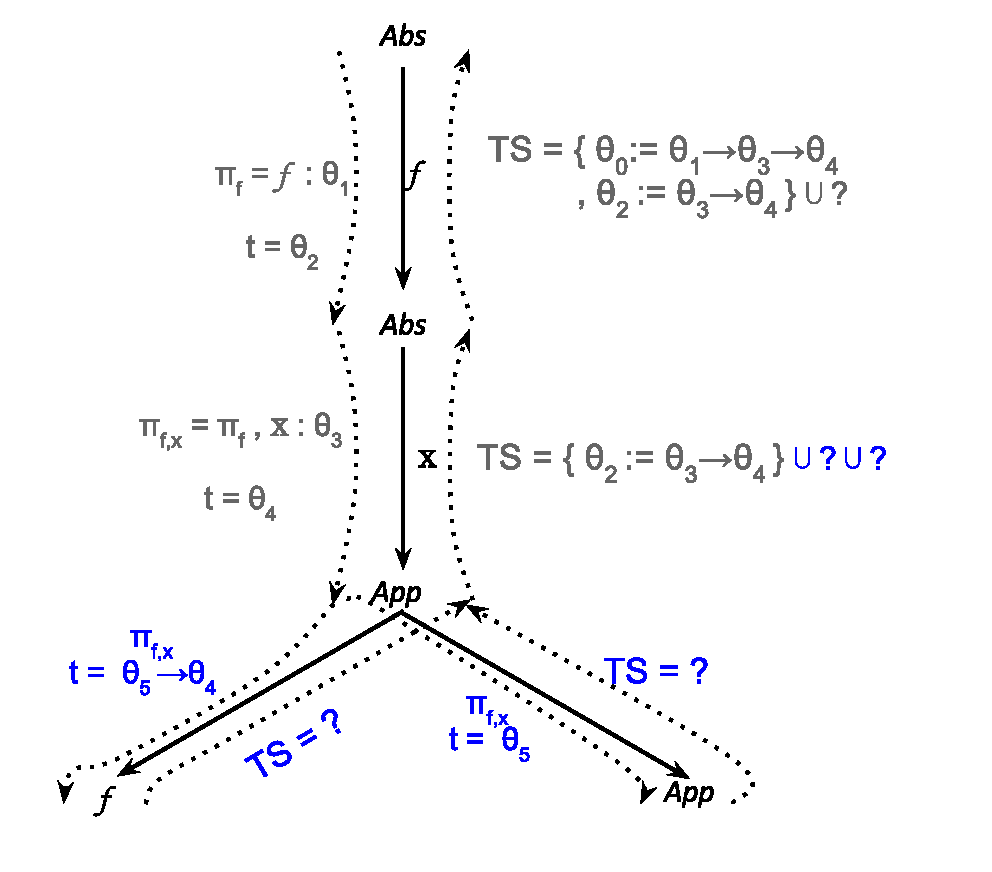
\includegraphics[height=10cm]{./tercero.pdf}
\end{center}

  La substitución en una aplicación será la unión de las de los subtérminos, por eso todavía no la completamos
  \medskip

  Ahora tenemos dos términos que analizar. El izquierdo es el identificador con la variable $f$ y el tipo asumido es
  $\theta_5 \rightarrow \theta_4$, pero en el contexto tenemos la información $f:\theta_1$ entonces agregamos
  a la substitución $\theta_1 := \theta_5 \rightarrow \theta_4$. 
  
  En el término derecho de la aplicación tenemos otra aplicación con el tipo $\theta_5$, entonces realizamos el mismo
  procedimiento:
  
\begin{center}
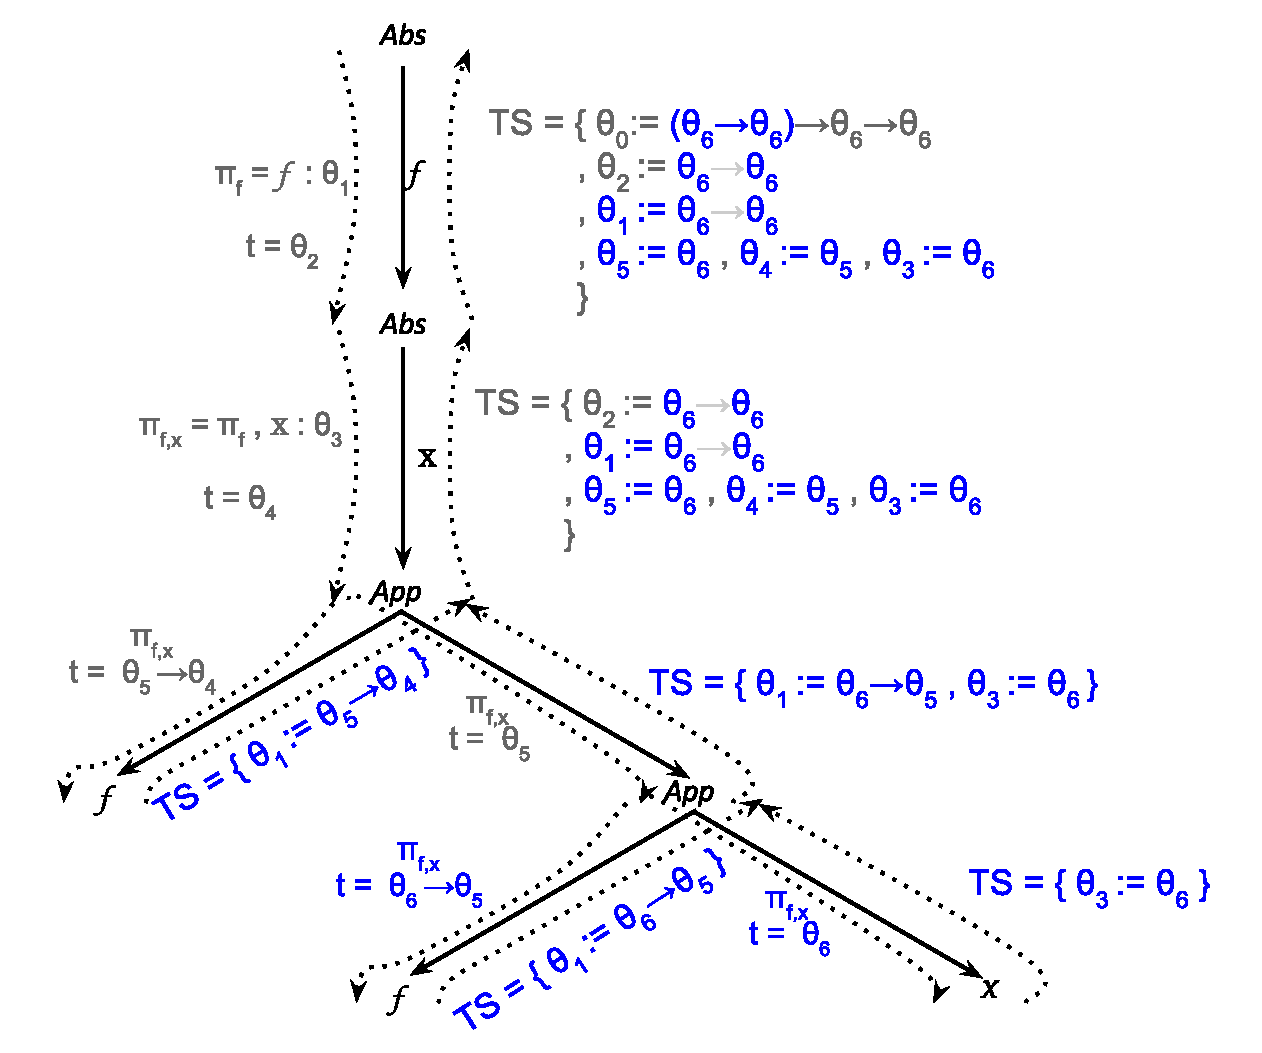
\includegraphics[height=10cm]{./cuarto.pdf}
\end{center}
   
  Ahora tenemos de nuevo en el lado izquierdo el identificador $f$ y el tipo asumido es $\theta_6 \rightarrow \theta_5$,
  y como en el contexto tenemos $f:\theta_1$ agregamos a la substitución $\theta_1 := \theta_6 \rightarrow \theta_5$.
  
  Al momento de concatenar las substituciones vemos que tenemos 
  
  
  
  
   
\end{document}




